\documentclass{exam}

\usepackage{units} 
\usepackage{graphicx}
\usepackage[fleqn]{amsmath}
\usepackage{cancel}
\usepackage{float}
\usepackage{mdwlist}
\usepackage{booktabs}
\usepackage{cancel}
\usepackage{polynom}
\usepackage{caption}
\usepackage{fullpage}
\usepackage{xfrac}
\usepackage{enumerate}

\newcommand{\degree}{\ensuremath{^\circ}} 
\everymath{\displaystyle}

\printanswers

% \begin{figure}[H]
%   \centering
%   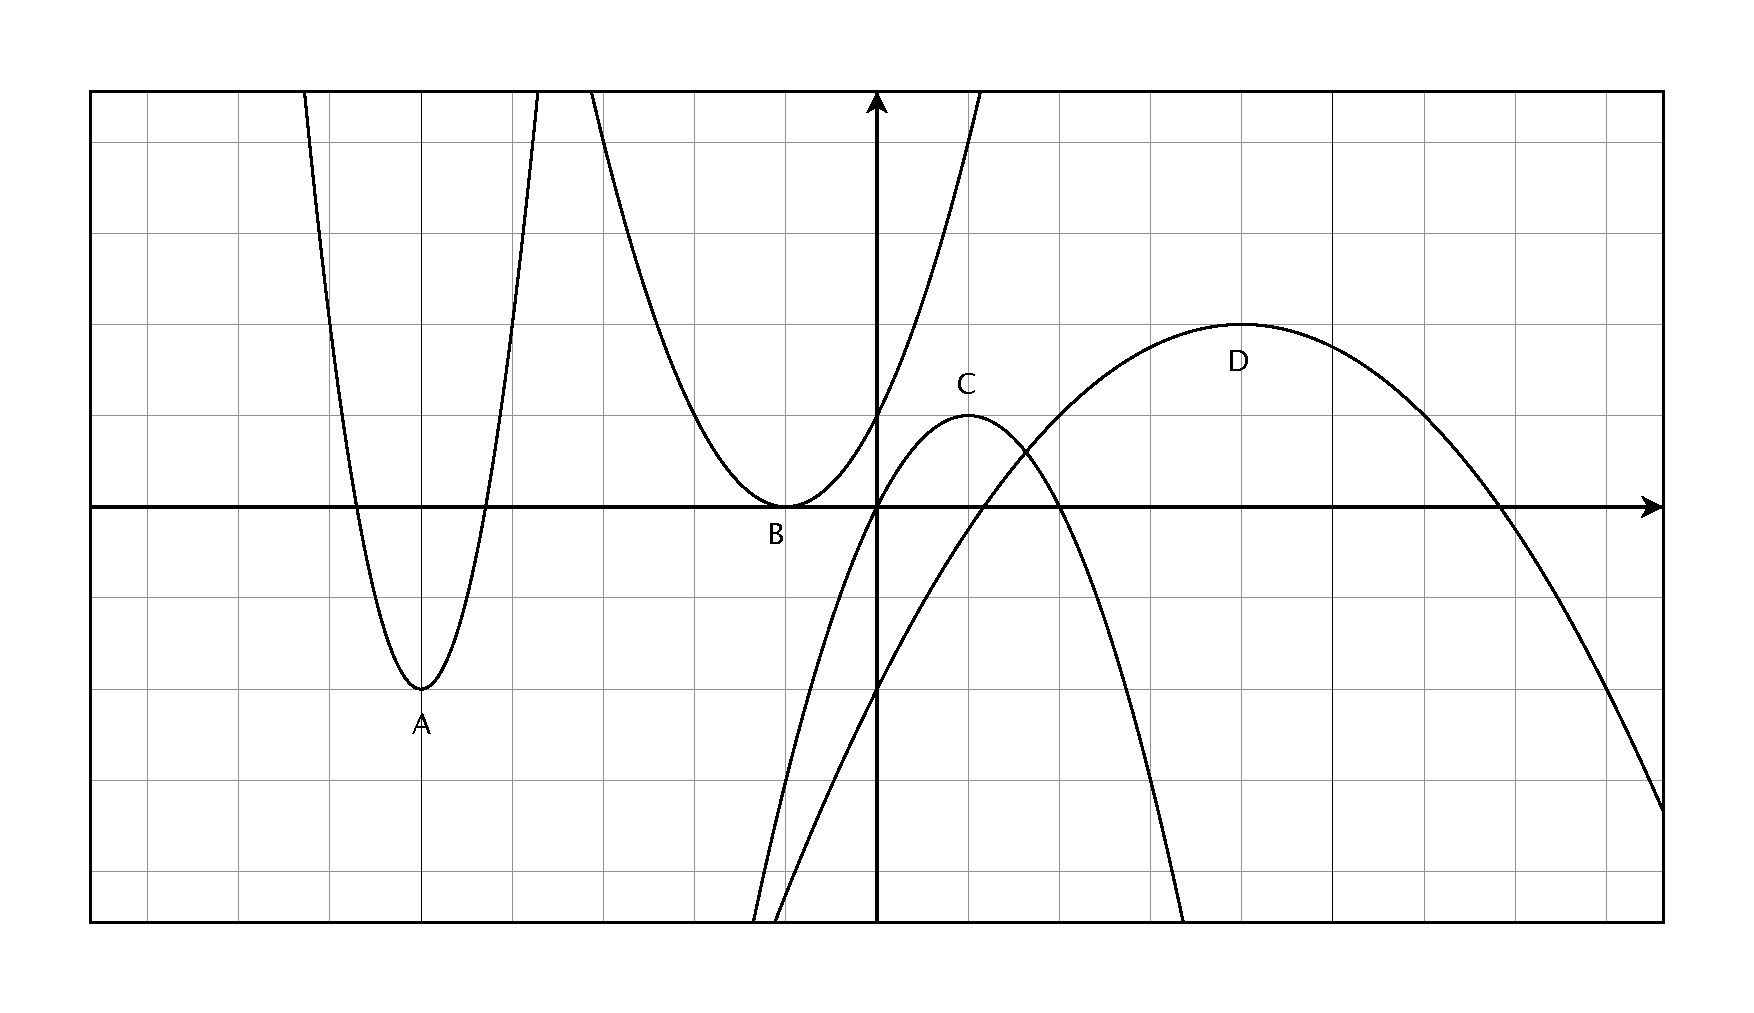
\includegraphics[scale=.3]{problem_7.eps}
%   \caption*{Problem 7}
% \end{figure}

% \begin{tabular}{cc}
% \toprule
% period & amplitude \\
% \midrule
%   $\pi$ & $2$ \\
% \bottomrule
% \end{tabular}

\title{Math 141 Notes \\ Section 4.3}

\date{June 19, 2013}

\begin{document}

  \maketitle
  \tableofcontents

  \section{Rules of Exponents}

  \subsection{Rules}
  \begin{align*}
    x^a \cdot x^b        &= x^{a + b} \\
    \frac{x^a}{x^b}      &= x^{a - b} \\
    \left( x^a \right)^b &= x^{ab} \\
  \end{align*}

  \section{Rules of Logarithms}

  \begin{align*}
    m &= b^x \\
    x &= \log_b m \\
    \\
    n &= b^y \\
    y &= \log_b n \\
  \end{align*}

  multiplying
  \begin{align*}
    \log_b \left( mn \right) &= \log_b \left( b^x \cdot b^y \right) \\
                             &= \log_b b^{x + y} \\
                             &= x + y \\
                             &= \log_b m + \log_b n \\
  \end{align*}

  dividing
  \begin{align*}
    \log_b \left( \frac{m}{n} \right) &= \log_b \left( \frac{b^x}{b^y} \right) \\
                             &= \log_b b^{x - y} \\
                             &= x - y \\
                             &= \log_b m - \log_b n \\
  \end{align*}

  powers
  \begin{align*}
    \log_b m^z &= \log_b \left( b^x \right)^z \\
               &= \log_b b^{xz} \\
               &= xz \\
               &= z \log_b m \\
  \end{align*}

  \subsection{Examples}

  \begin{enumerate}
    \item $\log_4 \sqrt[5]{64} = \frac{3}{5}$

    \item $\log_2 48 - \log_2 3 = \log_2 16 = 4$

    \item $\log 50 + \log 20 = \log 1000 = 3$

    \item 
      \begin{align*}
        \log_4 80 - \log_4 5 &= \log_4 \frac{80}{5} \\
                             &= \log_4 16 \\
                             &= 2 \\
      \end{align*}

    \item
      \begin{align*}
        \log_{15} 25 + \log_{15} 9 &= \log_{15} 225 \\
                                   &= 2 \\
      \end{align*}

    \item $\log(2x)$

    \item $\log \frac{x}{2}$

    \item $\log(x^3)$

    \item $\log(x^3 y^2)$

    \item $\log \frac{x^3 \sqrt{y}}{2}$

    \item $\log 2 + \log 3$

    \item $2 \log x - \log (x - 1)$

  \end{enumerate}

  \section{Change of Base}

  If you know logarithms in some base (base a) you can find logarithms in any other base (base b):
  \begin{align*}
    y          &= \log_b x \\
    b^y        &= x \\
    \log_a b^y &= \log_a x \\
    y \log_a b &= \log_a x \\
    y          &= \frac{\log_a x}{\log_b x} \\
    \log_b x   &= \frac{\log_a x}{\log_b x} \\
  \end{align*}

  \subsection{Examples}

  \begin{enumerate}
    \item $\log_5 17 = \frac{\ln 17}{\ln 5}$ 
    \item etc.
  \end{enumerate}
\end{document}
